\documentclass[11pt, a4paper, reqno, captions=tableheading,bibliography=totoc]{scrartcl}

\usepackage[utf8]{inputenc}
\usepackage[T1]{fontenc}
\usepackage{mathtools}
\usepackage{amsthm}
\usepackage{amsmath}
\usepackage{amssymb}
\usepackage{lmodern}
\usepackage[english]{babel}
\hyphenation{ei-gen-scheme}
\usepackage{booktabs}
\usepackage{float}
\usepackage{enumitem}
\usepackage{tikz,pgf}
%\usepackage[utopia]{mathdesign}
\usepackage{palatino}
\usepackage{hyperref}
\hypersetup{
    colorlinks,
    linkcolor={red!50!black},
    citecolor={blue!50!black},
    urlcolor={blue!80!black}
}
\usepackage[nameinlink]{cleveref}
\usepackage{xcolor}

\theoremstyle{plain}
\newtheorem{lemma}{Lemma}[section]
\newtheorem{prop}[lemma]{Proposition}
\newtheorem{theorem}[lemma]{Theorem}
\newtheorem*{theoremnonr}{Theorem}
\newtheorem{corollary}[lemma]{Corollary}
\newtheorem{conjecture}[lemma]{Conjecture}
\newtheorem{fact}[lemma]{Fact}
\newtheorem{assumption}[lemma]{Assumption}
\newtheorem*{reduction}{Reduction}
\theoremstyle{definition}
\newtheorem{definition}[lemma]{Definition}
\newtheorem{es}[lemma]{Example}
\newtheorem*{notation}{Notation}
\newtheorem{rmk}[lemma]{Remark}


\newcommand{\N}{\mathbb{N}}
\newcommand{\Z}{\mathbb{Z}}
\newcommand{\Q}{\mathbb{Q}}
\newcommand{\R}{\mathbb{R}}
\newcommand{\C}{\mathbb{C}}
\newcommand{\p}{\mathbb{P}}
\newcommand{\sP}{\mathcal{P}}
\newcommand{\sL}{\mathcal{L}}
\newcommand{\de}{\partial}
\newcommand{\codim}{\mathrm{codim}}

\newcommand{\oo}{\mathcal{O}}
\newcommand{\Bl}{\mathrm{Bl}}

\newcommand{\iso}{\mathcal{C}_{\mathrm{iso}}}

\newcommand{\imunit}{i}

\newcommand{\SO}{\operatorname{SO}}
\newcommand{\Eig}[1]{\mathcal{E}\!\left( {#1} \right)}
\newcommand{\Sym}{\operatorname{Sym}}
\newcommand{\polq}{{\rm Pol}_Q}
\newcommand{\comment}[1]{}

\newcommand{\scl}[2]{\left\langle {#1}, {#2} \right\rangle}

\newcommand\scalemath[2]{\scalebox{#1}{\mbox{\ensuremath{\displaystyle #2}}}}

\newcommand{\iii}{\textbf{i}}
\definecolor{MyDarkGreen}{cmyk}{0.7,0,1,0}
\newcommand{\blue}[1]{{\color{blue}  [#1]}}
\newcommand{\cbc}{\ensuremath{\mathcal{C}}}
\newcommand{\rk}{\ensuremath{\mathrm{rk}}}


\title{Eigenpoint collinearities of plane cubics}
\author{Valentina Beorchia$^{\circ}$ \and Matteo Gallet$^{\diamond}$ \and Alessandro Logar}
\date{}

\renewcommand{\thefootnote}{\fnsymbol{footnote}}

\linespread{1.15}
\setlength{\parindent}{0pt}
\setlength{\parskip}{.25em}

\begin{document}

\maketitle
\footnotetext{\hspace{0.15cm}$^\circ$ The researcher is a member of ``Gruppo Nazionale per le Strutture Algebriche, Geometriche e le loro Applicazioni'', INdAM. She is partially supported by MUR funds: PRIN project GEOMETRY OF ALGEBRAIC STRUCTURES: MODULI, INVARIANTS, DEFORMATIONS, PI Ugo Bruzzo, Project code: 2022BTA242.
\\
$^\diamond$ The researcher is a member of ``Gruppo Nazionale per le Strutture Algebriche, Geometriche e le loro Applicazioni'', INdAM.
}

\begin{abstract}
 Given a homogenous polynomial in $n+1$ variables, the fixed points of the map from $\p^n$ to itself given by its gradient are called the \emph{eigenpoints} of the polynomial. We focus on cubic polynomials in three variables, which have already been object of study regarding their eigenpoints, and study configurations of eigenpoints that admit one of more alignments. We give a classification of all possible configurations with alignments: this is accomplished using both geometric characterizations of these situations and an extensive use of computer algebra.
\end{abstract}

\section{Introduction}

Tensors are natural generalizations of matrices in higher dimension, and can be studied via their eigenvectors. There are several notions of eigenvalues and eigenvectors of tensors, as introduced independently in 2005 by Lim \cite{Lim} and Qi \cite{Qi}. All of them are of interest in several applications, like in the study of hypergraphs and the dynamical systems governed by those, see \cite[Section 4]{QZ} for an introduction or \cite{GMV} for recent developements. Eigenvalues of tensors also play an important role in the best rank-one approximation problem, which is relevant in data analysis and signal processing. As an example, consider the problem of maximizing a polynomial function $f$ over the unit sphere in $\R^{n+1}$: eigenvectors of the symmetric tensor $f$ are critical points of this optimization problem. Another interesting framework in which eigenvectors of symmetric tensors arise is the variational context: by Lim's Variational Principle \cite{Lim}, given a symmetric tensor $f$, the critical rank one symmetric tensors for $f$ are exactly of the form $v^d$, where $v$ is an eigenvector of $f$.
This has applications in low-rank approximation of tensors (see \cite{OttSod}) as well as maximum likelihood estimation in algebraic statistics.
The geometry of eigenpoints is intimately related with the Waring decomposition of a polynomial,
corresponding to the symmetric Tucker decomposition of the associated symmetric tensor,
as clearified in \cite{DOT} and in \cite{Ott}. Indeed, any best rank $k$ approximation of a symmetric tensor lies in the linear
space, called {critical space},  spanned by the rank $1$ tensors of the type $v_i ^{\otimes d}$, where $v_i$ vary among all the eingevectors. Therefore, a better comprehension of the geometry of the subschemes of an eigenscheme may lead to an improvement on the insight of low rank approximation problems. A first evidence in this direction is given by the so-called ODECO (orthogonally decomposable) tensors, that is symmetric tensors $T$ which admit a decomposition
$T= \sum _{i=0}^n v_i ^{\otimes d}$ with $v_0, \dotsc, v_n$ an orthogonal family; see \cite{Rob} and \cite{BDHE}
for further details. The $v_i$'s turn out to be eigenvectors of $T$. Finally, in \cite{OO} Oeding and Ottaviani employ eigenvectors of tensors to produce an algorithm to compute Waring decompositions of homogeneous polynomials.

In this extended abstract, we focus on symmetric tensors, i.e., homogeneous polynomials and in particular on ternary cubics.
In this setting, a ternary cubic~$F$ gives rise to a map $\nabla(F) \colon \p^2 \rightarrow \p^2$.
Proportional classes of eigenvectors of~$F$ are the fixed points of~$\nabla(F)$ and are called \emph{eigenpoint} of~$F$.
Therefore, the eigenpoints of~$F$ are the zeros of the $2 \times 2$ minors of the matrix
%
\begin{equation}
\label{eq:def_matrix_general}
    \begin{pmatrix}
    x & y & z \\
    \partial_x F & \partial_y F & \partial_z F
    \end{pmatrix} \,.
\end{equation}
%
Hence, the set of eigenpoints can be given a natural structure of determinantal scheme, which is commonly called an \emph{eigenscheme}, denoted $\Eig{T}$.

The dimension and degree of a general eigenscheme of a ternary cubic are in particular settled by the following result (see \cite[Theorem 2.1]{CartSturm} and \cite{Abo}): for a general $F \in \C[x, y, z]_3$, the eigenscheme $\Eig{F}$ is zero-dimensional, reduced and consists of $7$ points. Moreover, by \cite[Theorem 5.1]{ASS}, a configuration of seven points in $\p^2$ is the eigenconfiguration
of a ternary cubic if and only if no six of the seven points lie on a conic. Moreover, if $\Eig{F}$ contains two triples of aligned points, those must share a point. Finally, \cite[Theorem 5.7]{BGV} shows that the eigenscheme $\Eig{F}$ of a general homogeneous cubic polynomial $F \in \C[x, y, z]_3$ contains no $3$ collinear points.

The main results of this extended abstract are:
%
\begin{itemize}
\item the discussion of the algebraic and geometric conditions imposed by the existence of an aligned triple of eigenpoints (\Cref{conditions});
\item the classification of all possible configurations of alignments of the $7$ points constituiting a reduced, zero-dimensional eigenscheme of a ternary cubic (\Cref{alignments});
\item the classification of positive-dimensional eigenschemes of a ternary cubic (\Cref{positive_dimensional});
\item the computation of the degree of the locus of ternary cubics with one alignment in the eigenscheme    (\Cref{degree}).
\end{itemize}


\section{Invariance under the action of orthogonal matrices}
\label{invariance}

In what follows, it will be useful to fix particular coordinates for points and lines related to eigenschemes. To do that, we employ a property of invariance of eigenschemes with respect to the action of the following group.

\begin{definition}
 We define $\mathrm{SO}_3(\mathbb{C})$ to be the complexification of the group of special orthogonal real matrices, namely
 %
 \[
  \mathrm{SO}_3(\mathbb{C}) :=
  \bigl\{
   M \in \mathrm{GL}_3(\C) \, \mid \,
   M M^t = I_3 \  \text{and} \  \det(M) = 1
  \bigr\} \,.
 \]
 %
 The group $\mathrm{SO}_3(\mathbb{C})$ acts on $\C^3$ by matrix multiplication:
 %
 \[
  \begin{array}{ccc}
   \mathrm{SO}_3(\mathbb{C}) \times \C^3 & \rightarrow & \C^3 \\
   (M, v) & \mapsto & Mv
  \end{array}
 \]
 %
 Since all the elements of $\mathrm{SO}_3(\mathbb{C})$ are invertible, the latter action descends to an action on $\p^2(\C)$.
 Moreover, the group~$\mathrm{SO}_3(\mathbb{C})$ acts also on ternary forms via
 \[
  M \cdot F(x,y,z) = F(M^{-1} \cdot \prescript{t} {}( x \ y \ z )  ).
 \]
\end{definition}

A conic that will play a prominent role in our discussion if the so-called \emph{isotropic conic}, namely, the conic $\iso \subset \p^2$ of equation $x^2 + y^2 + z^2 = 0$. The action of $\mathrm{SO}_3(\mathbb{C})$ on $\p^2(\C)$ has two orbits: $\iso$ and $\p^2(\C) \setminus \iso$. Finally, the following result is well known.

\begin{prop}
 Let $M \in \mathrm{GL}_3(\C)$ and let $F$ be a ternary cubic.
 Let $P = (A: B: C)$ be a point in~$\p^2$.
 Then we have
 %
 \[
  P \in \Eig{F}
  \quad \text{if and only if} \quad
  M \cdot \prescript{t} {}(A \ B \ C) \in \Eig{M \cdot F}.
 \]
 %
\end{prop}

When proving a statement about eigenpoints $P_1, \dotsc, P_n$, the above results imply that it suffices to consider the two cases $P_1 = (1:0:0)$ and $P_1 = (1:\iii:0)$.

\section{Conditions imposed by aligned eigenpoints}
\label{conditions}

\subsection{The matrix of conditions}

Imposing a cubic ternary form to have one or more aligned triples of eigenschemes implies conditions both on the points and on the cubics.
We begin to explore these conditions by introducing, for each point $P \in \p^2$,
a $3 \times 10$ matrix encoding the condition that $P$ is an eigenpoint of a ternary cubic.

\begin{definition}
\label{definition:matrix_conditions}
 Consider $\p^9 = \p(\C[x,y,z]_3)$, the space of all ternary cubics.
 For $F \in \C[x,y,z]_3$, denote by $[F]$ the corresponding point in~$\p^9$; we denote by $w_F$ the (column) vector of coordinates of~$F$ (with respect to the standard lexicographic monomial basis of $\C[x,y,z]_3$). Then $w_F$ is also a vector of projective coordinates of~$[F]$.
 For a point $P = (A: B: C) \in \p^2$, the condition on elements~$[F]$ of~$\p^9$ that $P$ is an eigenpoint of the ternary cubic form~$F$ can be expressed in the form
 %
 \[
  \Phi(P) \cdot w_F
  = 0 \,,
 \]
 %
 where $\Phi(P)$ is a $3 \times 10$ matrix with entries depending on $A, B, C$.
 The matrix $\Phi(P)$ is called the \emph{matrix of conditions} imposed by~$P$.
We denote by $\phi_1(P)$, $\phi_2(P)$, and~$\phi_3(P)$ the rows of~$\Phi(P)$.
Moreover, if $P_1, \dotsc, P_n$ are points in the plane, we denote by $\Phi(P_1, \dotsc, P_n)$ the $3n \times 10$ matrix obtained by vertically stacking the matrices of conditions of~$P_1, \dotsc, P_n$.
\end{definition}

Tt is not difficult to check that the rank of $\Phi(P)$ is never $\leq 1$. Moreover
\begin{equation}
  C \, \phi_1(P) - B \, \phi_2(P) + A \, \phi_3(P) = 0 \,,
  \label{eq:base}
\end{equation}
therefore, among the three vectors, exactly two of them are linearly independent and the matrix~$\Phi(P)$ has rank~$2$.

\subsection{Possible ranks of the matrix of conditions}

In what follows we want to study the possible values of the rank of the matrix of conditions
$\Phi(P_1, \dots, P_n)$ for several configurations of points $P_1, \dots, P_n$
(and several values of~$n$).
In particular, we will study the ideal~$J_k$ of order $k$ minors of the
involved matrix and we will deduce some bounds about the rank from the possible
decompositions of the ideal~$J_k$. Most of these computations will be done
with the aid of a computer algebra system. Nevertheless, in many cases,
the result cannot be reached just by brute force, but it is necessary to
make some preprocessing on the ideal~$J_k$. In particular, it turns out that
it is often convenient to first saturate the ideal~$J_k$ with respect to
the distinct point condition or that three of them are not aligned (when this is the
case). Another important simplification that we adopt sometimes, makes use
of the action of~$\SO_3(\C)$: thanks to it we can assume that one of
the point is either $(1: 0: 0)$ or $(1: \iii: 0)$.

\begin{definition}
\label{definition:sigma}
For $P_1 = (A_1: B_1: C_1)$ and $P_2 = (A_2: B_2: C_2)$ in $\p^2$, we set
%
\[
  \sigma(P_1, P_2) := \scl{P_1}{P_1} \scl{P_2}{P_2} - \scl{P_1}{P_2}^2 \,,
\]
%
where
%
\[
 \scl{P_1}{P_2} = A_1 A_2 + B_1 B_2 + C_1 C_2
\]
%
and similarly for the other quantities.
The form $\sigma$ is the discriminant of the intersection between the line $P_1+P_2$ and $\iso$.
\end{definition}


\begin{prop}
\label{proposition:three_aligned_ranks}
Let $P_1, P_2, P_3$ be three distinct aligned points of the plane and let
$r$ be the line passing through them. Then:
\begin{itemize}
\item $5 \leq \rk \ \Phi(P_1, P_2, P_3) \leq 6$;
\item
$\rk \ \Phi(P_1, P_2, P_3) = 5$ if and only if $r$ is tangent
to~$\iso$ in one of the three points $P_1, P_2$, or $P_3$.
\end{itemize}
\end{prop}

We now define three quantities depending on a triple or on a $5$-tuple of points in the plane.
These quantities are crucial to describe what happens when we have aligned eigenpoints.
In the following, we denote by $P + Q$ the line through two distinct points $P$ and $Q$.

\begin{definition}
\label{definition:delta1}
 Let $P_1$, $P_2$ and~$P_4$ be distinct, not aligned points in the plane.
 We define the quantity
 %
 \[
  \delta_1(P_1, P_2, P_4) :=
  \scl{P_1}{P_1} \scl{P_2}{P_4} - \scl{P_1}{P_2}\scl{P_1}{P_4}
  =
  \scl{P_1\times P_2}{P_1 \times P_4} \,,
 \]
 %
 where $\times$ denotes the cross product, i.e.,
 %
 \[
  P_1 \times P_2 = (B_1 C_2 - C_1 B_2, \, C_1 A_2 - A_1 C_2, \, A_1 B_2 - B_1 A_2) \,.
 \]
 %
 and $P_1 = (A_1: B_1: C_1)$ and similarly for $P_2$ and $P_4$. Geometrically, the condition $\delta_1(P_1, P_2, P_4) = 0$ corresponds to the orthogonality of the vector planes corresponding to the lines $P_1 + P_2$ and $P_1 + P_4$.
\end{definition}

\begin{definition}
\label{definition:delta1b}
 Let $P_1$, $P_2$ and~$P_3$ be distinct aligned points in the plane.
 We define the quantity
 %
 \[
  \overline{\delta}_1(P_1, P_2, P_3) :=
  \scl{P_1}{P_1} \scl{P_2}{P_3} + \scl{P_1}{P_2}\scl{P_1}{P_3} \,.
  \]
 %
\end{definition}

\begin{definition}
\label{Vconf}
Let $P_1, P_2, P_3, P_4, P_5$ be five distinct points of the plane
such that $P_1, P_2, P_3$ and $P_1, P_4, P_5$ are aligned.
We call such a configuration a \emph{$V$-configuration}.
\end{definition}

\begin{definition}
 Let $P_1, \dots, P_5$ be a $V$-configuration.
We define the quantity
 %
 \[
  \delta_2(P_1, P_2, P_3, P_4, P_5) :=
  \scl{P_1}{P_2} \scl{P_1}{P_3} \scl{P_4}{P_5} -
  \scl{P_1}{P_4} \scl{P_1}{P_5} \scl{P_2}{P_3} \,.
 \]
 %
\end{definition}

\begin{theorem}
\label{theorem:rank_V}
Let $P_1, \dots, P_5$ be a $V$-configuration of
points. Then we have:
\begin{enumerate}
\item $8 \leq \rk \ \Phi(P_1, \dots, P_5) \leq 10$\,;
\item $\rk \ \Phi(P_1, \dots, P_5) \leq 9$ if and only if
$\delta_1(P_1, P_2, P_4) \cdot \delta_2(P_1, \dots, P_5) =0$\,;
\item $\rk \ \Phi(P_1, \dots, P_5) = 8$ if and only if, one of
the following two conditions is satisfied:
%
\begin{itemize}
\item $\delta_1(P_1, P_2, P_4) = 0$, \
$\overline{\delta}_1(P_1, P_2, P_3) = 0$,
\ $\overline{\delta}_1(P_1, P_4, P_5) = 0$\,;
  \item the line $P_1+P_2$ is tangent to~$\iso$ in $P_2$ or $P_3$
and the line $P_1+P_4$ is tangent to~$\iso$ in $P_4$ or $P_5$.
\end{itemize}
%
\end{enumerate}
\end{theorem}

We have that when the condition $\delta_2 = 0$ is met, another collinearity among the eigenpoints arises, indeed:

\begin{prop}
\label{proposition:terzo_allineamento}
If we have a $V$-configuration of five points $P_1, \dots, P_5$
such that the rank of the matrix $\Phi(P_1, \dots, P_5)$ is $9$ and
such that $\delta_2(P_1, \dots, P_5) = 0$,
then the unique cubic determined by the condition that $P_1, \dots, P_5$
are eigenpoints, has also the two other eigenpoints $P_6$ and $P_7$
aligned with $P_1$.
\end{prop}

To prove this statement, we combine several algebraic symbolic computations with the theory of Geiser maps.

\begin{definition}
The \emph{Geiser map} associated to a zero dimensional eigenscheme $\Eig{F}$ is the rational map defined by
%
\[
 \gamma_{\Eig{F}} \colon \p ^2 \dasharrow \p^2, \quad
 \gamma_{\Eig{F}} (P) = (G_1(P):G_2(P):G_3(P)) \,,
\]
%
where $G_1$, $G_2$, and $G_3$ are the order~$2$ minors of the matrix from \Cref{eq:def_matrix_general}.
\end{definition}

The key aspect that we need about Geiser maps is the following result.

\begin{lemma}
The Geiser map~$\gamma_{\Eig{F}}$ is surjective and its fiber over a point $Q = (a:b:c)$ is given by
%
\begin{equation}
\label{eq:fibers}
    \left\{
    \begin{array}{l}
    a x + by + cz = 0, \\[2pt]
    a \, \partial_x F + b \, \partial_y F + c \, \partial_z F = 0,\\
 \end{array}\right.
\end{equation}
%
that is, the intersection between the polar line $L_Q$ relative to the isotropic conic and $\mathrm{Pol}_Q F$, the
first polar curve of~$F$ with respect to~$Q$.

In particular, the only possible curves contracted by the Geiser map~$\gamma _{E(F)}$ are lines.
\end{lemma}

\begin{prop}
\label{proposition:P1_sing}
If $P_1, \dots, P_5$ is a $V$-configuration and if $\mathcal{C}$ is a cubic which
has $P_1, \dots, P_5$ among its eigenpoints, then $P_1$ is singular for~$\mathcal{C}$ if
and only if one of the following conditions is satisfied:
%
\begin{enumerate}
 \item $\delta_1(P_1, P_2, P_4) = 0$ and $\overline{\delta}_1(P_1, P_2, P_3) = 0$;
 \item $\delta_1(P_1, P_2, P_4) = 0$ and $\overline{\delta}_1(P_1, P_4, P_5) = 0$;
 \item $\overline{\delta}_1(P_1, P_2, P_3) = 0$ and
$\overline{\delta}_1(P_1, P_4, P_5) = 0$.
\end{enumerate}
%
\end{prop}

\section{Classification of possible alignments}
\label{alignments}

Here we provide the classification of all possible alignments of eigenpoints when the eigenscheme of a ternary cubic is zero-dimensional and reduced, hence it consists of~$7$ points.

\begin{figure}
 \centering
 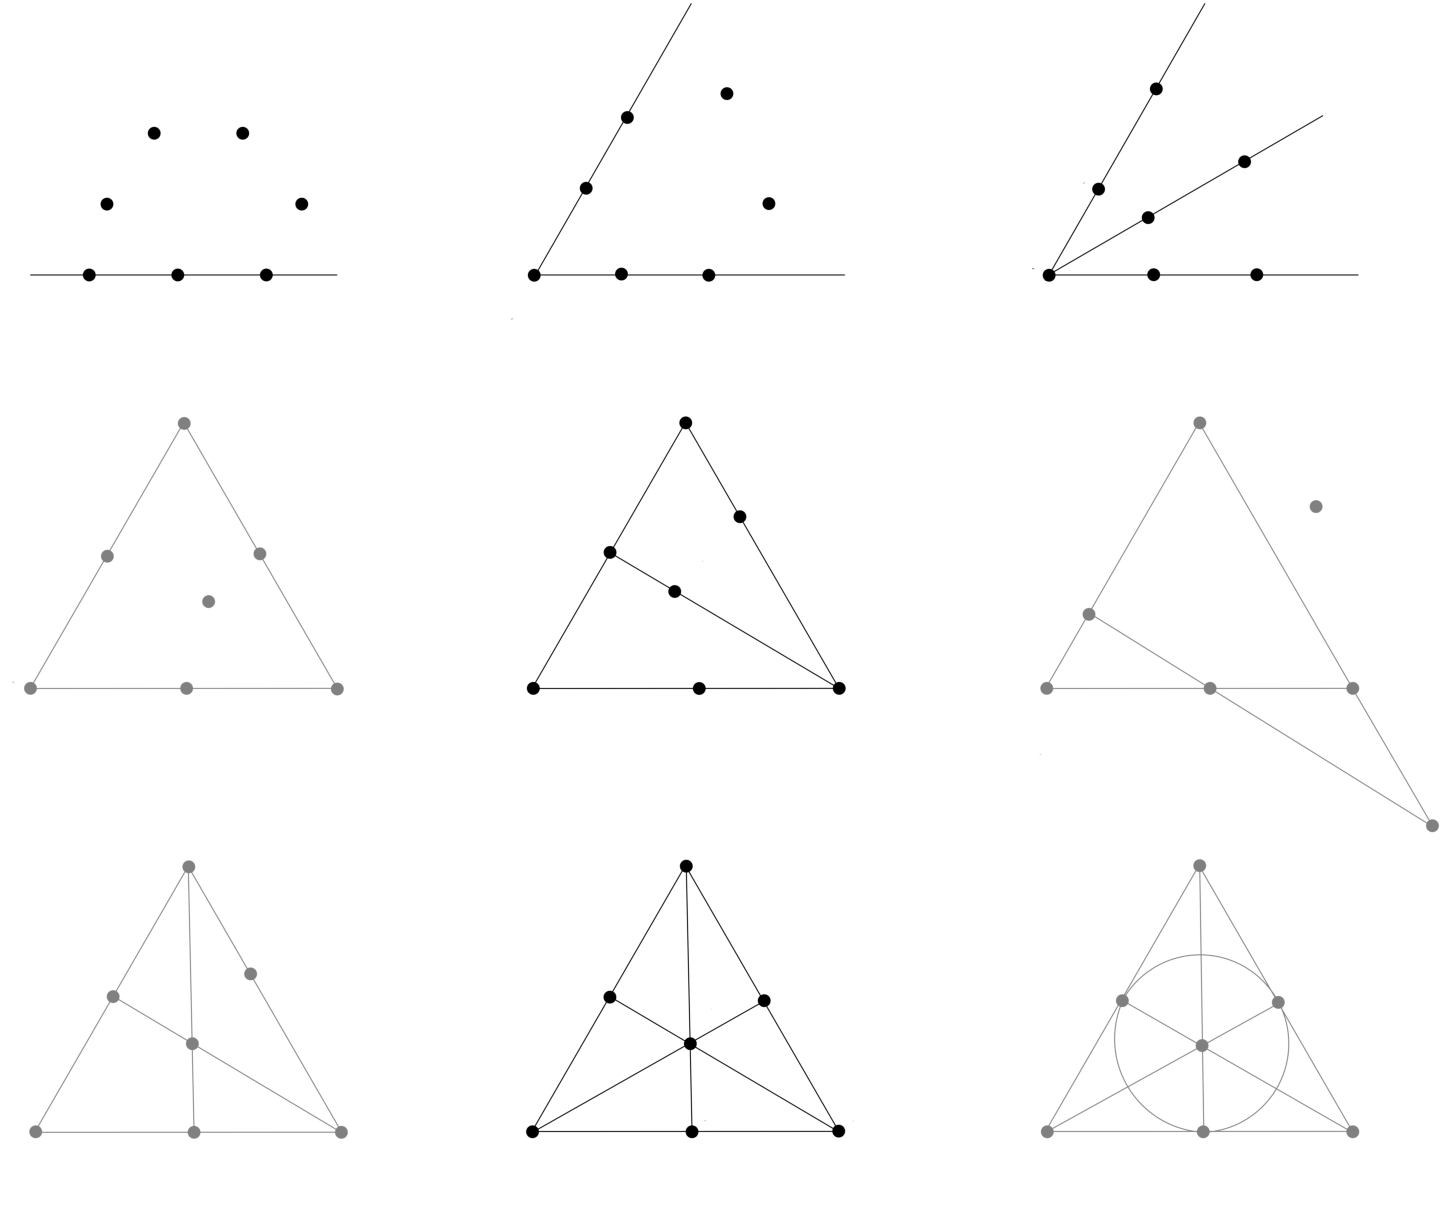
\includegraphics[trim={0.2cm 0 0.1cm 0}, width=\textwidth]{alignments}
 \caption{All nine possible combinatorial types of aligments of $7$ points. In black, those that arise as eigenpoints of a ternary cubic.}
 \label{figure:alignments}
\end{figure}


\Cref{figure:alignments} reports all possible $9$ combinatorial types of alignments of $7$ distinct points in the plane. Not all of them can be realized by eigenpoints of a ternary cubic.
This, again, follows from a careful analysis combining symbolic computations and the constraints obtained in the previous sections.

\section{Eigenschemes of positive dimension}
\label{positive_dimensional}

So far, we have focused on zero-dimensional eigenschemes of ternary cubics.
Here we classify all the situations of positive-dimensional ones.

We shall prove that residually we then have, in general, other three eigenpoints, and that the condition of having a line of eigenpoints is equivalent to having four collinear eigenpoints.

\begin{prop}
\label{p2}
Let $F$ be a ternary cubic.
Assume that $\dim \Eig{f} = 1$ and that the $1$-dimensional component is a line~$L$.
Then the residual subscheme $Z := \mathrm{Res}_L \bigl( \Eig{f} \bigr)$ in~$\Eig{f}$ with respect to~$L$ is zero-dimensional of degree~$3$.
\end{prop}
\begin{proof}
The proof relies in a careful discussion of the graded free resolution of the ideal sheaf of the scheme~$Z$, which is an almost complete intersection.
\end{proof}

\begin{es}
Consider the polynomial $F(x, y, z) = x^2 (y - z)$.
We have $L = x$,
%
\[
 H_1 = x^2-2y^2+2y z \,,
 \quad
 H_2 = 2z^2-x^2-2y z \,,
 \quad
 H_3 = 2yz-2z^2-xy \,.
\]
%
The two syzygies in degree~$3$ are:
%
\[
 z \, H_1 - y \, H_2 + x \, H_3 = 0 \,,
 \quad
 x \, H_2 + 2(y+z) \, H_3 + x \, H_1 = 0 \,.
\]
%
Finally, $Z = \bigl\{ (0:1:1), (2:1:-1), (-2:1:-1) \bigr\}$. Observe that one point is on the singular line $x = 0$
and that the Jacobian scheme is non reduced, it consists of a line with an embedded point.
\end{es}

\begin{prop}
\label{cubiche_con_2_rette}
Let $C$ be a cubic which has, among its eigenpoints, two lines $t_1$
and $t_2$. Then $t_1$ and $t_2$ are tangent to the isotropic conic
in two points $Q_1$ and $Q_2$ and, if $r$ is the line $Q_1+Q_2$
of equation $ax+by+cz=0$, the polynomial defining $C$ is:
\begin{equation}
C(r) = \left(r^2-3\left(a^2+b^2+c^2\right)\iso\right)r.
\label{2_lines_of_eigenpoints}
\end{equation}
$C$ has, in addition to $t_1$ and $t_2$, also the eigenpoint $(a: b: c)$
(the pole of $r$ w.r.t.\ $\iso$). \\
Conversely, if $C$ is defined by~(\ref{2_lines_of_eigenpoints}), where
$r$ is any line $ax+by+cz$ ($a, b, c \in K$), then
the eigenpoints of $C$ are the lines $t_1$ and $t_2$ (tangent to $C$
in the points $Q_1$ and $Q_2$ of intersection of $r$ with $\iso$) and
the point $(a: b: c)$.
\end{prop}


\begin{prop}
Given a line $t$ of the plane, if $t$ is not tangent to the isotropic
conic, then all the cubics which have, among their
eigenpoints, the points of $t$ are defined by the polynomial $r^2l$,
where $l$ is any line of the plane. If $t$ is tangent to $\iso$, then
all the cubics which have among their eigenpoints the points of $t$ are
defined by the polynomials
\begin{equation}
\label{cubiche_con_retta_autop_tg}
t^2l+\lambda C(r),
\end{equation}
where $\lambda \in K$ and $r$ is a line
passing through the tangent point $\iso\cap t$ (and $C(r)$ is defined
in~(\ref{2_lines_of_eigenpoints})). Conversely, if $r$ is a line and
$t$ is another line, tangent $\iso$ in one of the two points of intersections
of $r$ with $\iso$, then all the cubics given
by~(\ref{cubiche_con_retta_autop_tg}) have, among their eigenpoints,
the line $t$.
\end{prop}


\begin{prop}
Let $t$ be a line tangent to the isotropic conic in a point $P$. Then all the
cubics of the family~(\ref{cubiche_con_retta_autop_tg}) are singular in
$P$ and $t$ is one of the two tangents to the cubic in $P$.
\end{prop}

\begin{prop} All the cubics $C$ defined by the polynomial
\begin{equation}
\label{cub_conica_eig}
(\lambda \iso + \mu r^2)r \quad \mbox{$\lambda, \mu \in K$}
\end{equation}
where $r=ax+by+cz$ is a line of the plane,
have the eigenpoints given by the conic
$\lambda \iso+3\mu r^2$ (bitangent to $\iso$ in the points $\iso \cap r$)
and the point $(a:b:c)$ (the pole of $r$
w.r.t.\ $\iso$). Conversely, if
$C$ is a cubic of the plane which has a conic among its eigenpoints,
then there exists a line $r$ in the plane and $\lambda, \mu \in K$
such that the equation of
$C$ is given by~(\ref{cub_conica_eig}).
\end{prop}


\section{The degree of the variety of cubics with one alignment}
\label{degree}

The results of the previous sections allow one to determine the dimension and the degree of the locus of cubics having
at least one aligned triple of eigenpoints. We first recall a result by Abo concerning the locus of cubics with a non reduced or positive-dimensional eigenscheme.

\begin{definition}
An order $d$ tensor $T \in (\C^n)^{\otimes d}$ is called \emph{regular} if $\Eig{T} \subset \p^{n-1}$ is reduced of dimension $0$.
We set
%
\[
\Delta_{n,d}:=\{[T]\in \p ((\C^n)^{\otimes d}) \ | \ \Eig{T} \textrm{\ is \ not \ regular} \}\subset \p ((\C^n)^{\otimes d}) \,.
\]
%
The algebraic set~$\Delta_{n,d}$ is called the \emph{eigendiscriminant} (see \cite[Definition~5.5]{Abo}.
\end{definition}

\begin{theorem}(\cite[Corollary 5.8]{Abo})
The eigendiscriminant $\Delta_{n,d}$ is an irreducible hypersurface of degree $n(n-1)(d-1)^{n-1}$.
\end{theorem}

When restricting to symmetric tensors, the previous statement is still valid, as they form a linear subspace of
$\p \bigl((\C^n)^{\otimes d}\bigr)$ and the generic symmetric tensor has a regular eigenscheme.

In the particular case $n=d=3$, we have that the eigendiscriminant hypersurface has degree~$24$.

\begin{definition}
Let $\mathcal{U} \subset \p^9$ be the following locus:
%
\[
\mathcal{U} := \{[F]\in \p^9 \setminus \Delta_{3,3} \ | \ \Eig{F} \ \textrm {contains \ a \ unique \ aligned \ triple}\},
\]
%
and define $\mathcal{L} \subseteq \p^9$ as the closure of $\mathcal{U}$:
%
\[
 \mathcal{L} := \overline{\mathcal{U}} \subset \p^9.
\]
%
\end{definition}

We are now going to compute the degree of~$\mathcal{L}$.

\begin{prop}
 If $F, G \in \p^9 \setminus \Delta_{3,3}$ are general cubics, then any cubic in the pencil $\lambda F + \mu G$ for $(\lambda: \mu) \in \p^1$ has at most one aligned triple of eigenpoints.
\end{prop}

\begin{definition}
 Given a ternary cubic~$F$, we denote by $\Lambda_F$ the net of cubics whose base locus is the eigenscheme~$\Eig{F}$.
\end{definition}

\begin{lemma}
\label{lemma:scroll}
 If $F$ and $G$ are general cubics, then
 %
 \[
   \mathcal{N} := \bigcup_{(\lambda : \mu) \in \p^1} \Lambda_{\lambda F + \mu G} \subset \p^9
 \]
 %
 is an embedding of a rational projective bundle and has degree~$3$.
\end{lemma}

\begin{theorem}
The degree of $\mathcal{L}$ is equal to~$15$.
\end{theorem}
\begin{proof}
We start by observing that a reduced $0$-dimensional eigenscheme of a ternary cubic~$F$ contains an aligned triple if and only if the net of cubics $\Lambda_F$ contains a cubic which splits in three lines, a so called \emph{triangle}. Moreover, if $F$ is general enough, we have exactly one aligned triple and the other $4$ points are in general position; in this case, the net $\Lambda_F$ contains exactly three triangles, namely the unions of the line passing through the aligned triple and the reducible conics through the $4$ points in general position.

To determine the degree of $\mathcal{L}$ we consider a general pencil of cubic forms $\lambda F + \mu G$, and we compute the number of elements with associated net $\Lambda_{\lambda F + \mu G}$ containing a triangle. To this aim, denote by $\mathcal{T} \subset \p^9$ the variety of triangles; it is a classical result that its dimension is $6$ and its degree is $15$, see for instance \cite[Section 2.2.2]{3264}. We consider the variety~$\mathcal{N}$ from \Cref{lemma:scroll}.
Note that, since each net containing a triangle, actually contains exactly $3$ of them, the number of nets of $\mathcal{N}$ containing some triangle is given by
%
\[
\frac{\mathcal{T} \cdot {\mathcal N}}{3} = \frac{{15} \cdot {3}}{3} = 15 \,.
\]
%
This implies that $\deg \mathcal{L} = 15$.
\end{proof}


\bibliographystyle{amsalpha}
\bibliography{biblio}

\bigskip
\bigskip

\textsc{(Valentina Beorchia) University of Trieste,
Department of Mathematics, Informatics and Geosciences,
Via Valerio 12/1, 34127 Trieste, Italy}\\
Email address: \texttt{beorchia@units.it}

\textsc{(Matteo Gallet) University of Trieste,
Department of Mathematics, Informatics and Geosciences,
Via Valerio 12/1, 34127 Trieste, Italy}\\
Email address: \texttt{matteo.gallet@units.it}

\textsc{(Alessandro Logar) University of Trieste,
Department of Mathematics, Informatics and Geosciences,
Via Valerio 12/1, 34127 Trieste, Italy}\\
Email address: \texttt{logar@units.it}

\end{document}
